
\documentclass[a4paper]{article}
\usepackage{interlude}
\usepackage{pslatex}
\usepackage[T1]{fontenc}
\usepackage[utf8]{inputenc}
\setlength\parskip{\medskipamount}
\setlength\parindent{0pt}
\usepackage{graphicx}
\usepackage{amssymb}
\usepackage{tikz}
\usepackage{verbatim}
\usepackage{multicol}
\usepackage{fixltx2e}
\usepackage{amsmath}
%\usepackage{hyperref}

\makeatletter

\newcommand{\parent}			{\supset}
\newcommand{\child}			{\subset}
\newcommand{\master}			{\leftarrowtail}
\newcommand{\slave}			{\rightarrowtail}
\newcommand{\OSC}[1]		{\texttt{#1}}
\newcommand{\variete}			{\ensuremath{\mathcal{V}}}

\newenvironment{inscore}	{\vspace{-2mm}\small\verbatim}{\endverbatim\vspace{-2mm}}

\tikzstyle{box}=[rectangle,draw,fill=white!50,text=black] 
\tikzstyle{child}=[->,very thick,>=latex]
\tikzstyle{childD}=[->,dotted,very thick,>=latex]


\setlength{\parskip}{1mm}

\makeatother

\begin{document}

\title{Graphic rendering of synchronized objects specification \\ v.1.04}


\author{Grame \\ Centre national de cr\'eation musicale}

\maketitle

%=============================================== INTRO ===================================================
\section*{Introduction}\label{sec:intro}

An augmented music score is a graphic space that supports music scores and arbitrary graphic resources, including real-time elements, and providing time synchronization between all the score components. Each of those elements possesses a time position and a mapping that bounds their graphical dimensions to the time space.

In a context of interaction between elements (and possibly in the future with other musical processes), we define two types of dependencies between elements : the hierarchy and the synchronization. The first one on a mainly graphical base, and the second one on a time base, influencing the graphical representation.

The aim of this specification is to define the behavior of multiple or chained synchronizations, involving objects with children and slaves.

%======================================== 2 TYPES OF RELATION ==========================================================
\section{Two types of relations between objects}\label{sec:relations}

In order to understand the problematics of graphic rendering for the synchronized objects, we should first try to describe the two possibilities of interaction between objects in an augmented score : the parent-child relation, and the master-slave relation. 

%-------------------------------------------------- Hierarchy ---------------------------------------------------
\subsection{Hierarchy (parent-child relation)}\label{subsec:hierarchy}

"A is parent of B" will be symbolized by : $A \parent B$

"B is child of A" will be symbolized by : $B \child A$

\bigskip

With the 1.04 version of INScore, any object of the scene can have children objects, each one corresponding to a subnode in their OSC address. 

This is a purely graphical relation : the child object is drawn by its parent and in its parent's relative coordinates. It has no meaning in the time space. 

As the hierarchy between objects defines their OSC path, we can therefore agree that a single object can only have a single parent (but several children). 

\bigskip

\begin{figure}[h]
\begin{center}
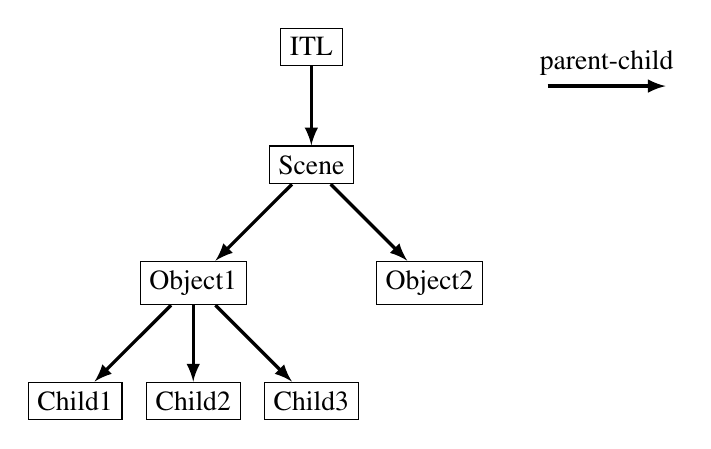
\begin{tikzpicture}

  \node[box] (I) at (0,3) {ITL};
  \node[box] (S) at (0,1.5) {Scene};
  \node[box] (O1) at (-1.5,0) {Object1};
  \node[box] (O2) at (1.5,0) {Object2};
  \node[box] (C1) at (-3,-1.5) {Child1};
  \node[box] (C2) at (-1.5,-1.5) {Child2};
  \node[box] (C3) at (0,-1.5) {Child3};
  
  \draw[child] (I)--(S);
  \draw[child] (S)--(O1); \draw[child] (S)--(O2);
  \draw[child] (O1)--(C1); \draw[child] (O1)--(C2); \draw[child] (O1)--(C3);
  % la légende
  \draw[child] (3,2.5)--(4.5,2.5)node[midway,above]{parent-child};
  
\end{tikzpicture}

 \caption{The parent-child hierarchy}
 \label{fig:hierarchy}

\end{center}
\end{figure}

%-------------------------------------------------- Synchronization ---------------------------------------------------
\subsection{Synchronization (master-slave relation)}\label{subsec:sync}

"A is master of B" will be symbolized by : $A \master B$

"B is slave of A" will be symbolized by : $B \slave A$
\bigskip

Time synchronization represents the possibility to graphically synchronize the augmented score components in order to align the graphic sections of the score components that correspond to equivalent time spaces. Each object on the augmented score has a time position and a duration. The other objects on its level of hierarchy (objects having the same parent) can then be synchronized on it, which means that they will be positioned, and possibly stretched, to fit their time position and duration relatively to their master's, and depending on the synchronization mode. 

Both of the slave and master objects should have their own time to graphic mapping, that can then be used to create a graphic to graphic mapping corresponding to the direct link between the two elements. 

A master can have several slaves and a slave several masters. Each master-slave relation should have its own options and behavior.


\begin{figure}[h]
\begin{center}

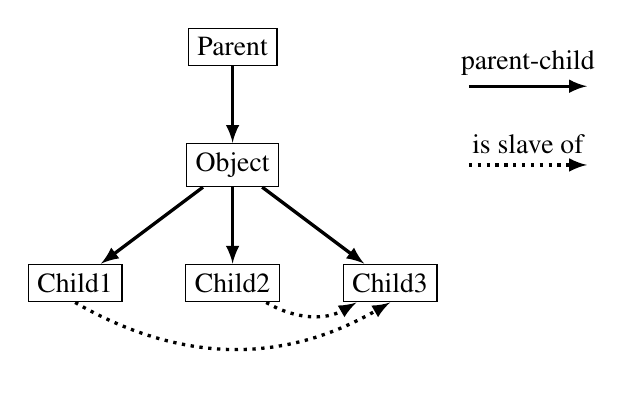
\begin{tikzpicture}

  \node[box] (P) at (0,3) {Parent};
  \node[box] (O) at (0,1.5) {Object};
  \node[box] (C1) at (-2,0) {Child1};
  \node[box] (C2) at (0,0) {Child2};
  \node[box] (C3) at (2,0) {Child3};
  
  \draw[child] (P)--(O);
  \draw[child] (O)--(C1); \draw[child] (O)--(C2); \draw[child] (O)--(C3);
  \draw[childD] (C2)to[bend right](C3); \draw[childD] (C1.south)to[bend right](C3.south);
  %
  \draw[child] (3,2.5)--(4.5,2.5)node[midway,above]{parent-child};
  \draw[childD] (3,1.5)--(4.5,1.5)node[midway,above]{is slave of};
    
 \end{tikzpicture}

 \caption{The slave-master synchronization}
 \label{fig:sync}

\end{center}
\end{figure}

This graphic to graphic mapping defines graphical segments in the slave (source) element, that will correspond to graphical segments in the master (destination) element.
The set of all those segments is called segmentation. Without specification, the default segmentation will be a unique segment corresponding to the object's bounding box.

In practice, the graphic to graphic mapping is built by calculating a list of pairs of graphical segments (or rectangles), each one of these pairs representing the path from the slave's to master's spaces.

\bigskip

The graphical segmentation of the object A will be represented by $Seg_A$

%The middle point of a graphical segment S will be represented by $m_S$

The bounding box of the object A will be represented by $S_A$

The time segmentation of the object A will be represented by $T_A$

The time to graphic mapping of the object A will be represented by $M_A = Seg_A \times T_A$

The graphic to graphic mapping of a synchronization between two elements will be represented by $M_{slave/master}$

The date (time position) of the object A will be represented by $t_A$ and its duration (time segment) by $d_A$.



%==================================== MULTIPLE SYNC ==============================================================
\section{Multiple synchronizations}\label{sec:multSync}

As said before, it is possible for a slave to have several masters. This means that it will be drawn as many times as the number of masters, and have as many mappings (a list of lists of pairs of rectangles !). The object's appearance will vary depending on its relation with each of its masters (stretch or not, placed on the top or on the bottom, in a relative or absolute time...).

\begin{inscore}
/ITL/scene/parent/sync child1 child2;
/ITL/scene/parent/sync child1 child3 h;
/ITL/scene/parent/sync child1 child4 hv;
\end{inscore}

%exemple avec partitions et curseur

\begin{figure}[h]
\begin{center}

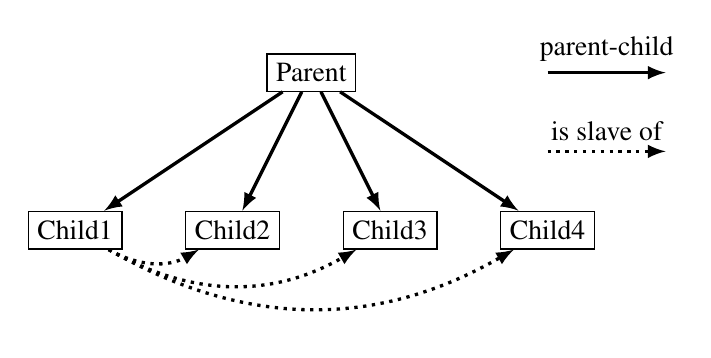
\begin{tikzpicture}

  \node[box] (P) at (0,2) {Parent};
  \node[box] (C1) at (-3,0) {Child1};
  \node[box] (C2) at (-1,0) {Child2};
  \node[box] (C3) at (1,0) {Child3};
  \node[box] (C4) at (3,0) {Child4};
  
  \draw[child] (P)--(C1); \draw[child] (P)--(C2); \draw[child] (P)--(C3); \draw[child] (P)--(C4);
  \draw[childD] (C1)to[bend right](C2); \draw[childD] (C1)to[bend right](C3); \draw[childD] (C1)to[bend right](C4);
  % 
  \draw[child] (3,2)--(4.5,2)node[midway,above]{parent-child};
  \draw[childD] (3,1)--(4.5,1)node[midway,above]{is slave of};
    
 \end{tikzpicture}

\caption{Example of multiple synchronization}
\label{fig:multipleSync} 
 
\end{center}
\end{figure}
   
\begin{figure}[h]
\centering


\includegraphics[width=5cm]{img/sync2.png}   	            
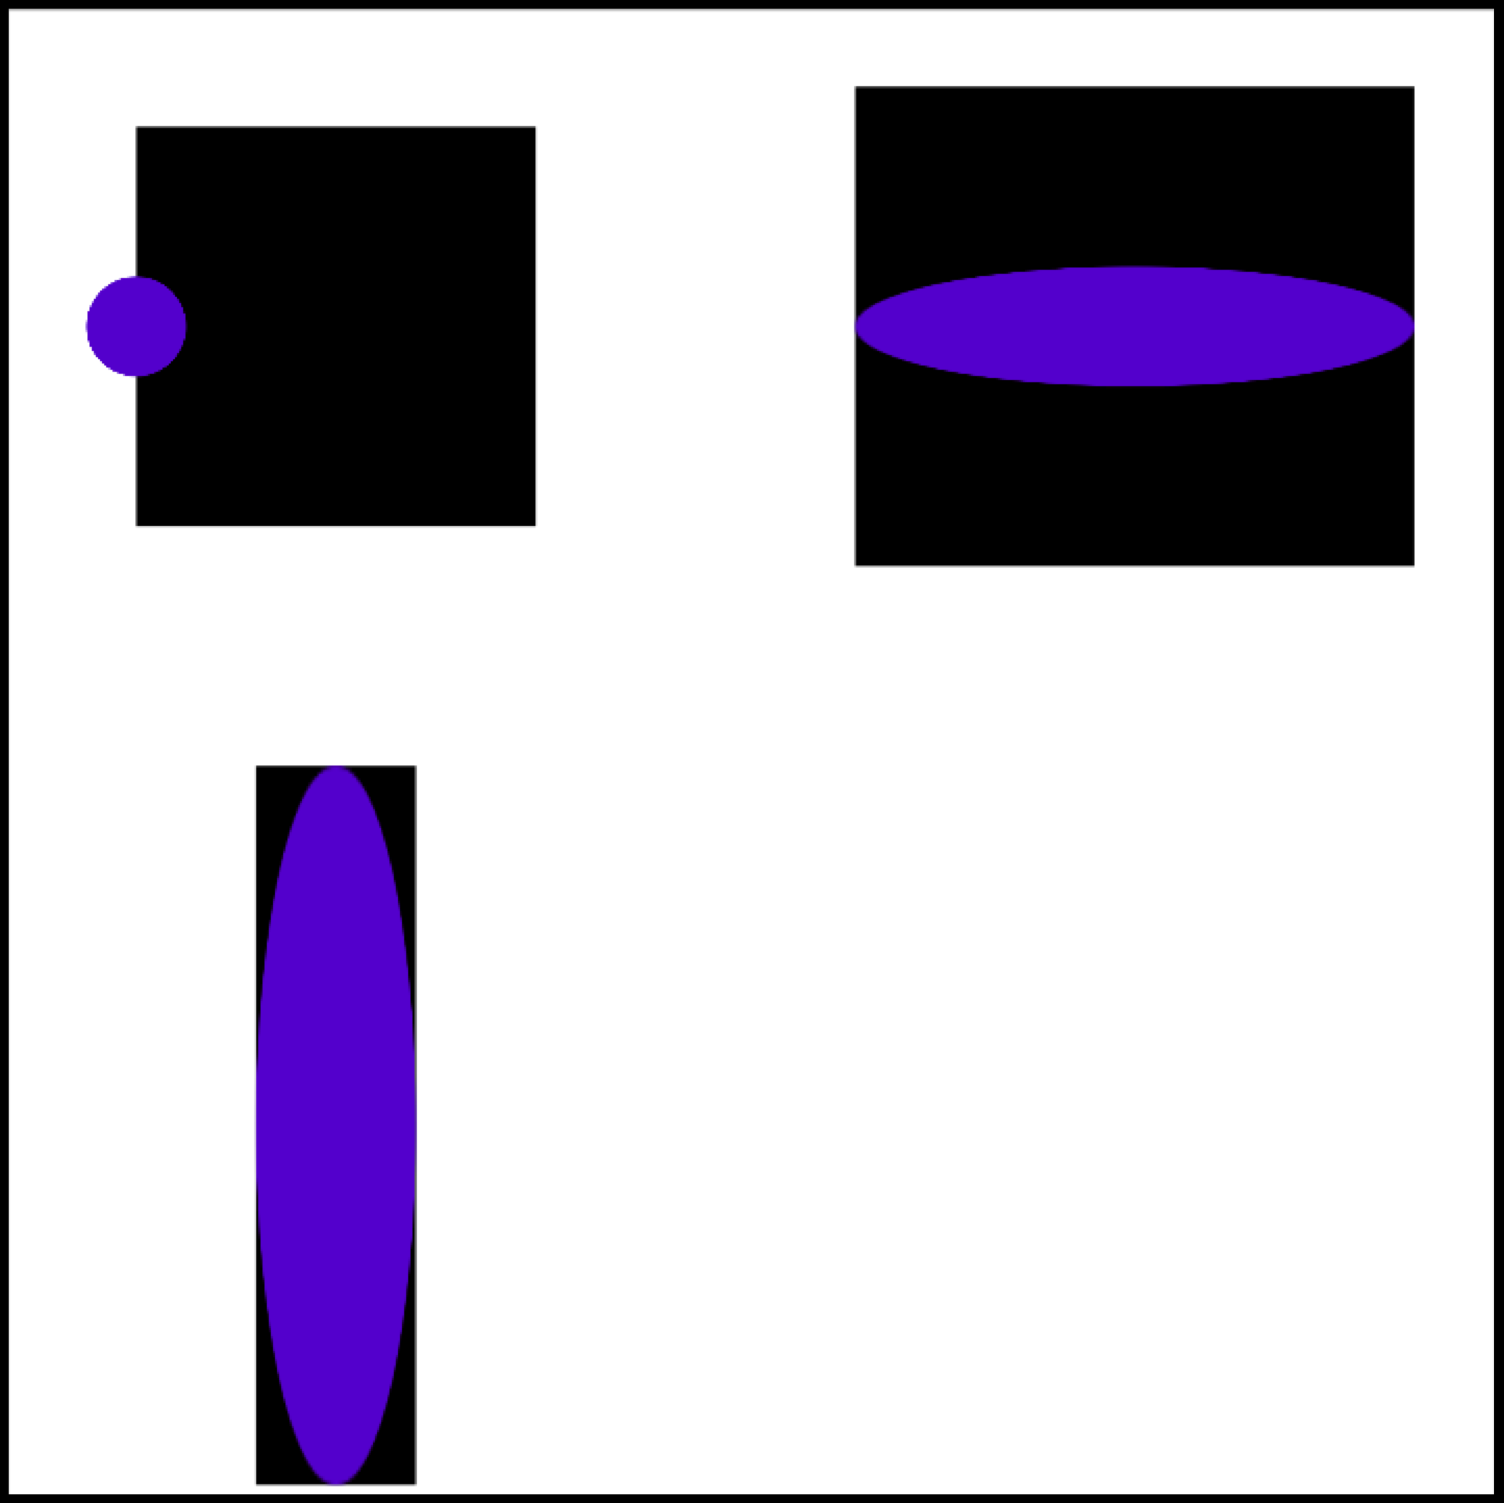
\includegraphics[width=5cm]{img/sync.png}
\caption{The purple circle is synchronized on the three other objects}
\label{fig:sync}
\end{figure}

%========================================== SYNC WITH CHILDREN AND SLAVES ========================================================
\section{Synchronization on objects with children or slaves}\label{sec:sync_children}

Now that we have defined the main characteristics of both graphic and time hierarchies, we should try to specify the behavior of synchronized objects, that themselves may have children and/or slaves : What should we do with those children and slaves ? Should they be drawn with their parent or master ? Should they be stretched with it ? Mapped ?
\\

The object A with all its children and slaves will be represented by \r{A}.
\\

Let's take the following case of an object B synchronized on a score A and having a slave C and children d, e and f. 
\\
\begin{figure}[h]
\centering
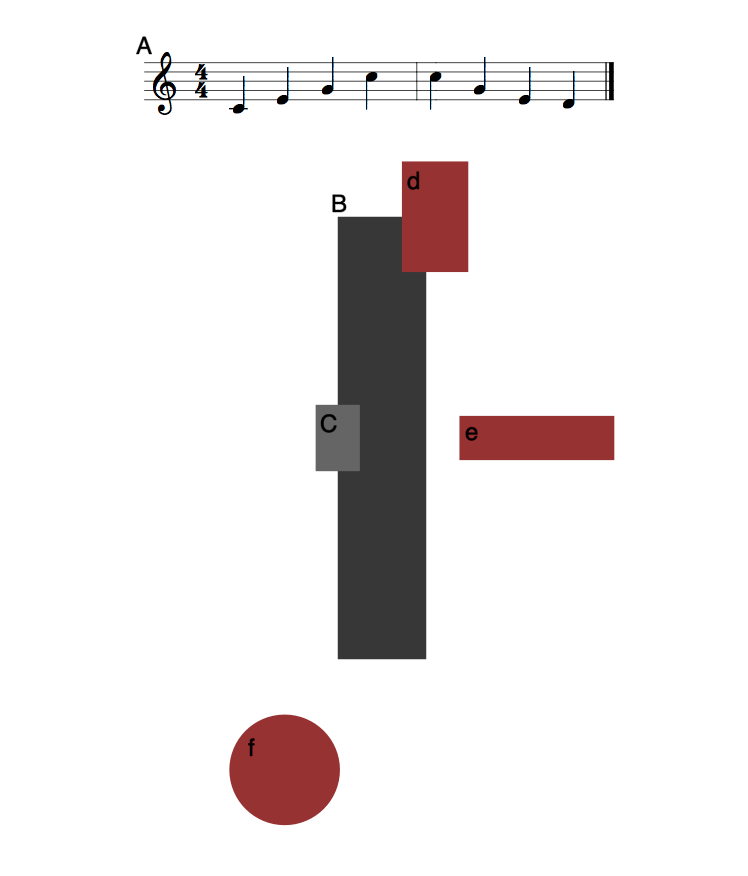
\includegraphics[width=8cm]{img/score.png}   	            
\caption{Synchronization of an object with children and slaves}
\label{fig:defaultMap}
\end{figure}

\begin{center}
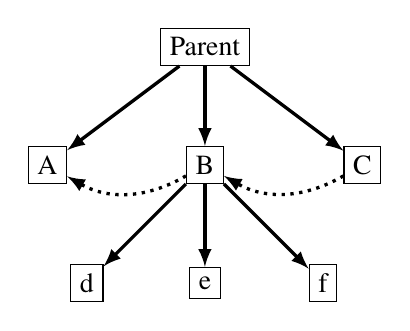
\begin{tikzpicture}
  \node[box] (P) at (0,3) {Parent};
  \node[box] (A) at (-2,1.5) {A};
  \node[box] (B) at (0,1.5) {B};
  \node[box] (C) at (2,1.5) {C};
  \node[box] (d) at (-1.5,0) {d};
  \node[box] (e) at (0,0) {e};
  \node[box] (f) at (1.5,0) {f};
  
  \draw[child] (P)--(A); \draw[child] (P)--(B); \draw[child] (P)--(C);
  \draw[child] (B)--(d); \draw[child] (B)--(e); \draw[child] (B)--(f);
  \draw[childD] (B)to[bend left](A);
  \draw[childD] (C)to[bend left](B);
\end{tikzpicture}
\end{center}

 $B \slave A$

 $B \parent (d, e, f)$

 $B \master C$



%-------------------------------------------------- Bounding Box---------------------------------------------------
\subsection{Bounding Boxes of parent and children}\label{subsec:bb}

First of all, we should define the rectangle $S\textsubscript{\r{B}}$ corresponding to the set of the object with its $n$ children and slaves. 

\begin{center} $ S\textsubscript{\r{B}}  =\{ \bigcup \limits_{i=1}^n S_i \} \bigcup S_B$ \end{center}

Note that the union of rectangles used here is defined in \cite{fober12cmj2} by the bounding box of all rectangles.% (figure \ref{fig:rectunion}).

\begin{figure}[h]
\centering
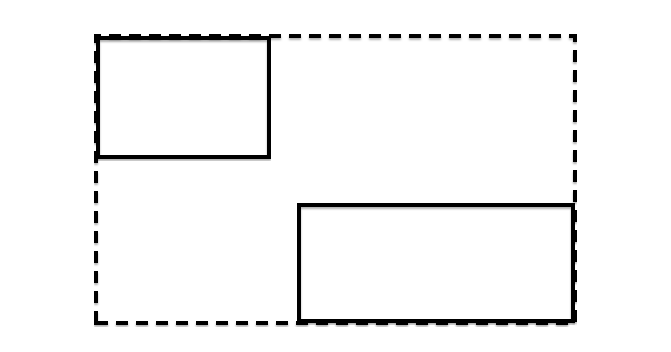
\includegraphics[width=40mm]{img/rect.png}
\caption{Union of two rectangles (graphical segments)}
\label{fig:rectunion}
\end{figure}

The children having the possibility of being drawn outside of their parent's bound, the general case is : 
\begin{center} $i \child B \nRightarrow S_i \subset S_B$ \hspace{0.2cm} and \hspace{0.2cm} $ S_B \subseteq S\textsubscript{\r{B}} $ \end{center}
%and so :
%\begin{center} $ S\textsubscript{\r{B}} \bigcap S_B \neq S\textsubscript{\r{B}}$  \end{center}

\begin{figure}[h]

\begin{multicols}{2}

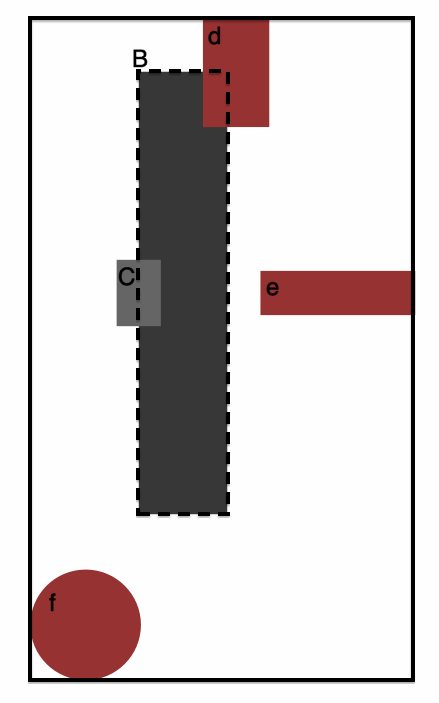
\includegraphics[width=4cm]{img/score3.png}   	            

\columnbreak

 - - - -  $S\textsubscript{B}$ %and its destination segment $S'\textsubscript{B}$

\bigskip

 ------  $S\textsubscript{\r{B}}$ %and its destination segment $S'\textsubscript{\r{B}}$

\bigskip

 $S\textsubscript{\r{B}} = \bigcup(S_B, S_A, S_C, S_d, S_e, S_f) $

\end{multicols}
\caption{The source graphical segments}
\label{fig:sync}
\end{figure}


%\begin{multicols}{2}
%
%\begin{tikzpicture}
%  \node[box] (P) at (0,1.5) {Parent};
%  \node[box] (A) at (-1.5,0) {A};
%  \node[box] (B) at (1.5,0) {B};
%  \node[box] (a) at (-3,-1.5) {a};
%  \node[box] (b) at (-1.5,-1.5) {b};
%  \node[box] (c) at (0,-1.5) {c};
%  
%  \draw[child] (P)--(A); \draw[child] (P)--(B);
%  \draw[child] (A)--(a); \draw[child] (A)--(b); \draw[child] (A)--(c);
%  \draw[childD] (B)to[bend left](A);
%\end{tikzpicture}
%
%\columnbreak
%
%A \supset (a, b, c)
%
%A \leftarrowtail B
%
%\r A  =  \bigcup (A, B, a, b, c)
%
%\end{multicols}

%-------------------------------------------------- Default mapping ---------------------------------------------------
\subsection{Case of the default mapping for the slave}\label{subsec:defaultMap}

In the case of a default mapping, $Seg_B = \{S_B\}$ . We are then dealing with a synchronization with no stretch or with a vertical stretch. 
\\

We know that the segment (or, in this case, bounding box) $S_B$ is linked, through a graphic to graphic mapping, to another segment $S'_B$ that depends on the master object A : 

\begin{center} $(S_B, S'_B) \in M_{B/A}$ with $M_{B/A} = Seg_B \times Seg_A$ \end{center}

The aim here is to define this segment $S'_B$, but also to find the corresponding segment $S'\textsubscript{\r{B}}$ linked to $S\textsubscript{\r{B}}$, the bounding box of \r{B}.

%-------------------------------------------------- variety  ---------------------------------------------------
\subsubsection{Variety of a segment}\label{subsubsec:variety}

To define our destination segments $S_B$ and $S'\textsubscript{\r{B}}$, we will appeal to the concepts of continuous mapping and variety .%\cite{fober:10b}.
\\

For $\theta : [0,1] \rightarrow [0,1]$ and $I = [a,b[$, we name variety of I, the set of points $\variete(I,\theta)$ from I defined by :
\begin{center}
$\variete(I, \theta) =  \lbrace (1 - \theta(t)).a + \theta(t).b \mid t \in [0, 1[ \rbrace$ 
\end{center}

Intuitively, the variety of an interval expresses the relationship between this interval and its variety using a function $\theta$ defined on $[0, 1[$.
\\
\begin{figure}[h]
\centering
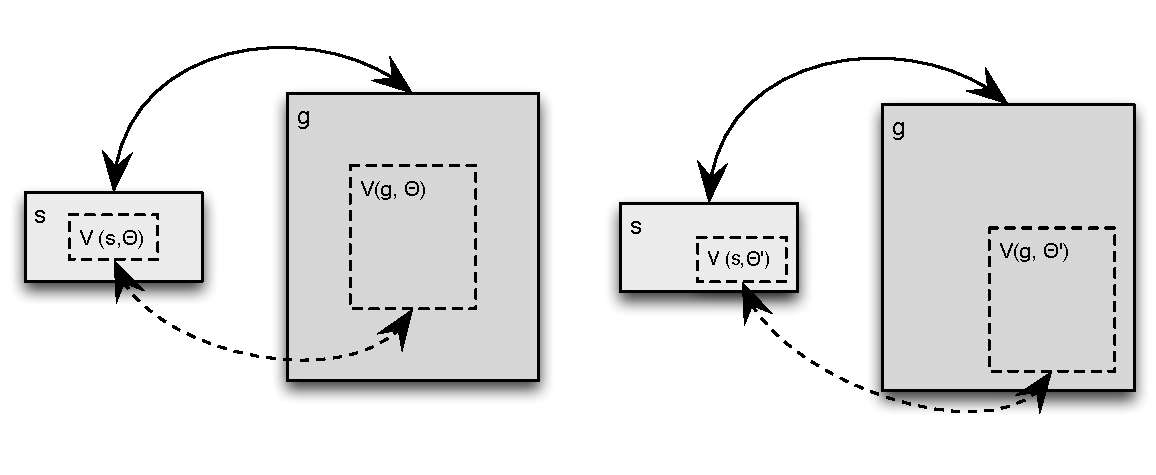
\includegraphics[width=11cm]{img/vmapping.pdf}
\caption{Varieties of two graphical segments}
\label{fig:variety}
\end{figure}
% référence : pas publiée ??

%-------------------------------------------------- destination rect ---------------------------------------------------
\subsubsection{Definition of $S'\textsubscript{B}$}\label{subsubsec:defDestRect}

%For now, we are in the case of a default mapping for the slave object. Looking for its destination segment can be seen as defining the master's default mapping.

Let's now remember that the INScore scene has time representation on its horizontal (x-axis) dimension. The vertical one being purely graphical.

If we look for the position and dimension of our destination segment $S'_B$, we should first try to find the relation between the time position of B, $t_B$, and an x-position in the mapping $M_A$. 

As long as we have a time segment $D_A$ in $T_A$ (the time segmentation) that contains the time position $t_B$, we know that we have a graphical segment $S_A$ in $Seg_A$ (the graphical segmentation) that will contain our slave's position. If there is no such segment in $T_A$, the slave will simply not be drawn.

\begin{figure}[h]
\begin{center}
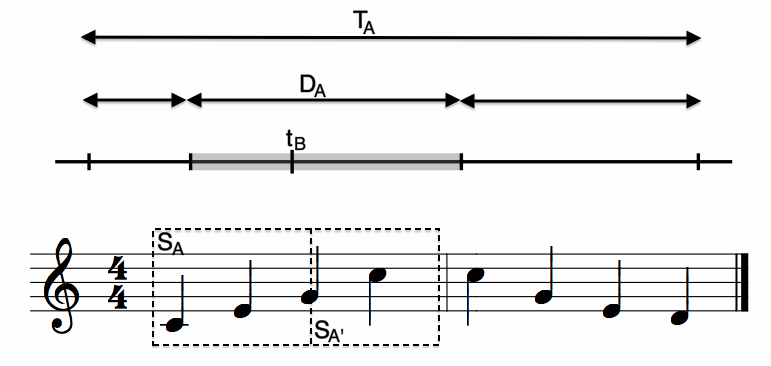
\includegraphics[width=9cm]{img/time_graphic4.png}
\caption{Relation between time and graphical mappings}
\label{fig:time2graphic}
\end{center}
\end{figure}

We can see the time position $t_B$ as a time segment $d_B = [t_B, t_B[$ that is a variety of $D_A$. We can then deduce a graphical segment $S'_A$ corresponding to the time segment $d_B$ :

\begin{center}
$d_B = \variete(D_A, \theta)$\\
$S'_A = \variete(S_A, (\theta, 1))$
\end{center}

This relation gives us a one-dimensional segment $S'_A$ with :
\begin{itemize}
  \item the x position corresponding to the time position $t_B$, 
  \item a null x dimension
  \item the y position centered on $S_A$
  \item and a y dimension corresponding to $S_A$'s height.
\end{itemize} 

% SCHEMA ?

In order to find our destination segment $S'_B$, we will define it as :
\begin{itemize}
  \item with its x origin position aligned on $S'_A$,
  \item with a x dimension corresponding to the source $S_B$ width,
  \item with y position and dimension depending on the vertical stretch and on the synchronization option "syncPos" (see Figure \ref{fig:possibleDestRect}).
\end{itemize}


$S'_B \mid \left\lbrace 
\begin{array}{lcl} 
x_{S'_B} = x_{S'_A}\\
\bigskip
width_{S'_B} = width_{S_B}\\
\bigskip
y _{S'_B} = \left\lbrace
\begin{array}{lcl}
y_{S_B} = y_{top_{S'_A}} - \hspace{1mm} height_{S_B}/2 & \text{if syncTop}\\ 
y_{S_B} = y_{S'_A} & \text{if syncOver}\\
y_{S_B} = y_{bottom_{S'_A}} + \hspace{1mm} height_{S_B}/2 & \text{if syncBottom}
\end{array}\right.\\
height _{S'_B} = \left\lbrace
\begin{array}{lcl}
height_{S_B} & \text{if no stretch}\\
height_{S'_A} & \text{if vertical stretch}
\end{array}\right.\\
\end{array}\right.$

\begin{figure}[h]
\begin{center}
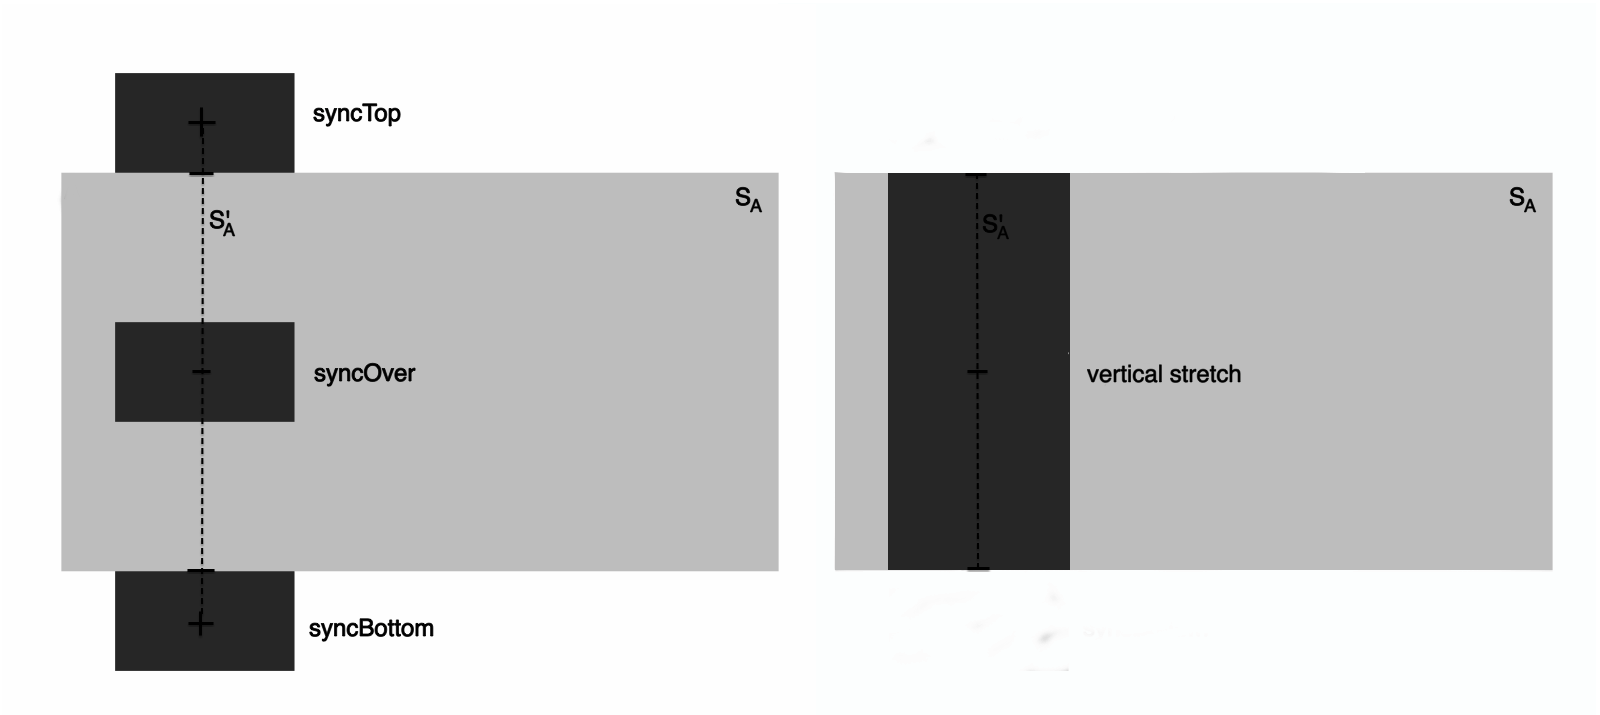
\includegraphics[width=16cm]{img/top_over_bottomF.png}
\caption{Different possibilities for the destination segment $S'_B$}
\label{fig:possibleDestRect}
\end{center}
\end{figure}


%-------------------------------------------------- destination rect with children ---------------------------------------------------
\subsubsection{Definition of $S'\textsubscript{\r{B}}$}\label{subsubsec:defDestChildRect}

We can see that, if we know $S_B$ (the object's bounding box) and $S\textsubscript{\r{B}}$ (the bounding box of the object and all its children and slaves), we can define the relation between them, that is the variety. 

Furthermore, the mapping $M_{B/A}$ gives us the destination segment $S'_B$, so we can deduce the segment $S'\textsubscript{\r{B}}$ by applying the same relation between $S'_B$ and $S'\textsubscript{\r{B}}$ than between $S_B$ and $S\textsubscript{\r{B}}$.
\\

for : \begin{center} $(S_B, S'_B) \in M_{B/A}$ and $M_{B/A} = Seg_B \times Seg_A$ \end{center}

we have :

\begin{center}
$(S\textsubscript{\r{B}}, S'\textsubscript{\r{B}}) \mid \left\lbrace 
\begin{array}{lcl} 
  S\textsubscript{\r{B}} \cap S_B = S_B\\ [0.2cm]
  \exists \theta \mid \left\lbrace
  \begin{array}{lcl}
    S_B = \variete(S\textsubscript{\r{B}}, \theta)\\% [0.5cm]
    S'_B = \variete(S'\textsubscript{\r{B}}, \theta)
  \end{array}\right.
\end{array}\right.$
\end{center}

\begin{figure}[h]
\begin{multicols}{2}
\begin{center}
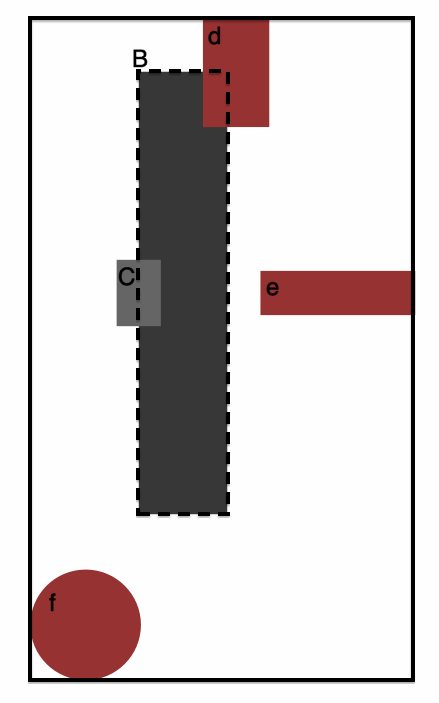
\includegraphics[width=5cm]{img/score3.png} 
\end{center}
\columnbreak

\bigskip

\begin{center}
 - - - -  $S\textsubscript{B}$ and its destination segment $S'\textsubscript{B}$

\bigskip

 ------  $S\textsubscript{\r{B}}$ and its destination segment $S'\textsubscript{\r{B}}$

\bigskip

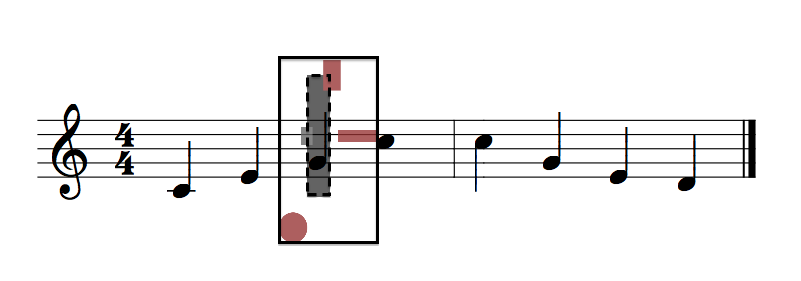
\includegraphics[width=9cm]{img/scorefinalbox.png}

\end{center}

\end{multicols}

\caption{The source and destination graphical segments}
\label{fig:mapping}

\end{figure}

%-------------------------------------------------- Case of stretching ---------------------------------------------------
\subsection{Case of stretching (the slave is mapped)}\label{subsec:complexMap}

In the case of a slave with mapping that should be stretched horizontally to fit its parent's mapping, it has been decided to take only into account the children that are in the object's bound.
As our object can be partially mapped, and so partially drawn in its master's mapping, there are no more reasons to extrapolate the drawing of its children than the drawing of the rest (not in the mapping) of the object itself.

\begin{figure}[h]
\begin{center}
\begin{multicols}{2}
source B:

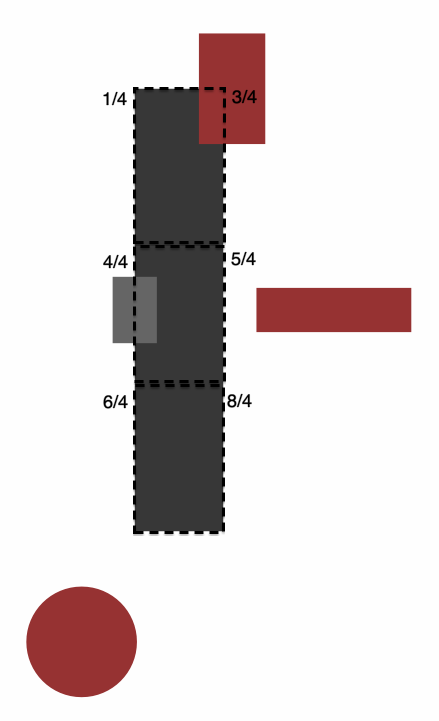
\includegraphics[width=6cm]{img/stretchB.png} 

\columnbreak
destination A: 
\vspace{10cm}
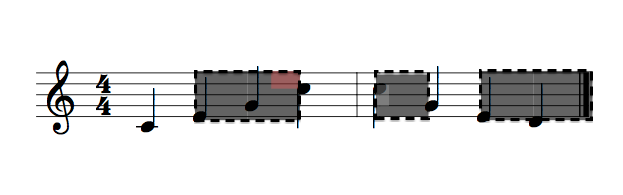
\includegraphics[width=9cm]{img/stretchA.png}

\end{multicols}
\caption{Case of a slave with mapping}
\label{fig:mapping}
\end{center}
\end{figure}

%-------------------------------------------------- Conclusion ---------------------------------------------------
%\section*{Conclusion}\label{sec:conclusion}
% conlusion ?

\bibliographystyle{unsrt}
\bibliography{interlude}

\end{document}
